\section{Controlling a Rockets Stability}
The previous design method does not provide a perfectly stable attitude control. Indeed to have such precise an active control system is necessary. Full scale rockets use the thrusting force to achieve such control. In order to do so most of them operate with the gimbaled thrust method. It consists of steering the engine's nozzle to get the thrusting force in right incidence, an example is seen cf. figure \ref{fig:RocketGimbal}. 
\begin{figure} [htbp]
	\centering
	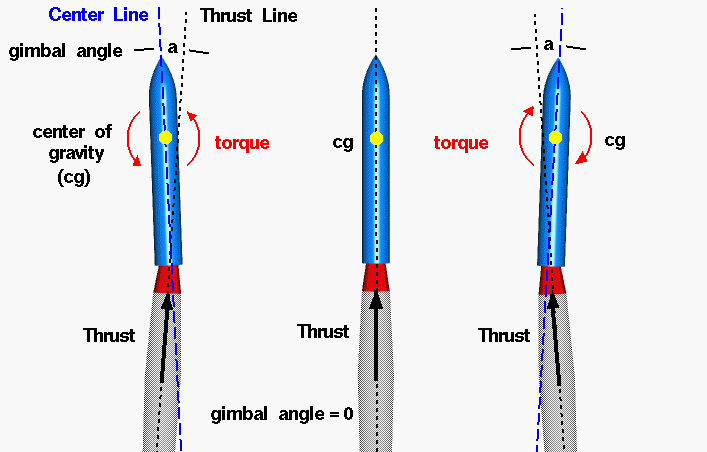
\includegraphics[width=0.8\linewidth]{RocketGimbal}
	\caption{Example of gimballing a rocket nozzle \cite{web:rocketnasa}.}
	\label{fig:RocketGimbal}
\end{figure}

Where a torque is applied to create a rotation around the rockets center of gravity. The thrust direction is relative to the position of the center of gravity.  This should compensate for direction deviations from the rockets center line or trajectory, and keep the rocket stable.    	

However Space X introduces a new propulsion method by using multiple small engines instead of a big one. With this method the thrusting force direction can be instead controlled by the output of each engine. For smaller rockets orientable fins are used. By changing the orientations of the fins the drag and the lift is changed and so is the attitude of the rocket.


Stabilization of rockets is therefore feasible with different types of control types. Most rockets is one time use which means that implementing and testing of a stabilization system would be high cost. Therefore will similar control systems be examined to research the possibility for making a ground based control system, which can be related to the motion and stabilization of a rocket in flight. 